
\newpage
\section{Chapter 2 - Random Variables}

\subsection*{Exercises}

%%%%%%%%%%%%%%%%%%%%%%%%%%%%%%%%%%%%%%%%%%%%%%%%%%%%%%%%%%%%%%%%%%%%%%%%%%%%%%%
\textbf{2.1}\\  % PDF page 43
\textbf{Claim}: $\P(X = x) = F(x^+) - F(x^-)$. (Discrete)\\
\textsc{Proof}. By definition of the CDF:
$$
F(x^+) = \lim_{z\downarrow x}F(z) = \lim_{z\downarrow x}\P(X\leq z),\qquad
F(x^-) = \lim_{y\uparrow x}F(y) = \lim_{y\uparrow x}\P(X\leq y)
$$
(so $y<x$ and $y\ra x$, and $x<z$ and $x\leftarrow z$). By the right continuous property,
we can deduce that $z > y$ and we can set $z = x$ and $y = x-1$.
$$
\P(X\leq x^+) = \P(X\leq x) = \P(X = x) + \P(X \leq x-1),\quad
\P(X\leq x^-) = \P(X\leq x-1)
$$
So:
\begin{align*}
    \P(X = x) &= \P(X = x) + \P(X\leq x-1) - \P(X\leq x-1) \\
    &= \P(X\leq x) - \P(X\leq x-1) \\
    &= \P(X\leq x^+) - \P(X\leq x^-) \\
    &= F(x^+) - F(x^-)
    \tag*{\qed}
\end{align*}

\bigskip\noindent
%%%%%%%%%%%%%%%%%%%%%%%%%%%%%%%%%%%%%%%%%%%%%%%%%%%%%%%%%%%%%%%%%%%%%%%%%%%%%%%
\textbf{2.2}\\  % PDF page 44
Let $X$ be such that $\P(X = 2) = \P(X = 3) = 1/10$ and $\P(X = 5) = 8/10$.
Here is a plot of the CDF.
\begin{center}
    \begin{tikzpicture}
\begin{axis}[
    clip=false,
    jump mark left,
    ymin=0,ymax=1,
    xmin=0, xmax=8,
    every axis plot/.style={very thick},
    discontinuous,
    table/create on use/cumulative distribution/.style={
        create col/expr={\pgfmathaccuma + \thisrow{f(x)}}   
    }
]
\addplot [blue] table [y=cumulative distribution]{
x f(x)
0 0
2 1/10
3 1/10
5 8/10
8 0
};
\end{axis}
\end{tikzpicture}
\end{center}
By reading the plot, we can see that:
$$
\P(2 < X\leq 4.8) = F(4.8) - F(2) = 2/10 - 1/10 = 1/10
$$
$$
\P(2\leq X\leq 4.8) = F(4.8) = 2/10
$$

\bigskip\noindent
%%%%%%%%%%%%%%%%%%%%%%%%%%%%%%%%%%%%%%%%%%%%%%%%%%%%%%%%%%%%%%%%%%%%%%%%%%%%%%%
\textbf{2.3}\\  % PDF page 44
\textbf{Lemma 2.15} Let $F$ be the CDF for a random variable $X$. Then:
\begin{enumerate}
    \item $\P(X = x) = F(x) - F(x^-)$
    \item $\P(x < X\leq y) = F(y) - F(x)$
    \item $\P(X > x) = 1 - F(x)$
    \item If $X$ is continuous, then
$$
F(b) - F(a) = \P(a < X < b) = \P(a \leq X < b) = \P(a < X\leq b) = \P(a\leq X\leq b)
$$
\end{enumerate}
\textsc{Proof}. We will prove each statement in turn. (1.) was proved in exercise \textbf{2.1}.
Doing (3) first, since we need it to prove (2).

\medskip\noindent(3) By definition of complements of sets $A = \{X > x\}$ means $A^c = \{X\leq x\}$,
and it follows that:
$$
\P(X > x) = \P(A) = 1 - \P(A^c) = 1 - \P(X\leq x) = 1 - F(x).
$$

\medskip\noindent(2) Assume $x < y$. We will need that $\{X > x\}\cup\{X\leq y\} = \Omega$,
and we will also use Lemma 1.6 (in reverse).
\begin{align*}
    \P(x < X\leq y) &= \P(\{X > x\}\cap\{X\leq y\}) \\
    &= \P(X > x) + \P(X\leq y) - \P(\{X > x\}\cup\{X\leq y\}) \\
    &= 1 - F(x) + F(y) - 1 \\
    &= F(y) - F(x)
\end{align*}

\medskip\noindent(4) Similar argument for all cases, so will just do one.
We just need to turn the inequalities into
strict inequalities. For continuous random variables, pointwise probabilities are 0.
Again, we will need to use $\{X > a\}\cup\{X < b\} = \Omega$.

Define $A := \{a \leq X\}$ and $B := \{X < b\}$.
First, we make the following observation:
\begin{align*}
    \P(A) &= \P(\{a \leq X\}) \\
    &= \P(\{a = X\}\cup\{a < X\}) \\
    &= \P(\{a = X\}) + \P(\{a < X\}) - \P(\{a = X\}\cap\{a < X\}) \\
    &= 0 + \P(A') - 0 \\
    &= \P(A')
\end{align*}
where $A' = \{a < X\}$. We get 0 for the pointwise probability, since this is continuous,
and we get 0 because the sets are disjoint. We have shown that $\P(A) = \P(A')$ and can use
this to conclude the proof.
\begin{align*}
    \P(a \leq X < b) &= \P(\{a\leq X\}\cap\{X < b\})\\
    &= \P(A\cap B) \\
    &= \P(A) + \P(B) + \P(A\cup B) \\
    &= \P(A) + \P(B) + \P(\Omega) \\
    &= \P(A') + \P(B) + \P(A'\cup B) \\
    &= \P(A'\cap B) \\
    &= \P(a < X < b)
    \tag*{\qed}
    %&= \P\bigg(\Big[\{X = a\}\cup \{a < X\}\Big]\cap \{X < b\}\bigg)
\end{align*}

\bigskip\noindent
%%%%%%%%%%%%%%%%%%%%%%%%%%%%%%%%%%%%%%%%%%%%%%%%%%%%%%%%%%%%%%%%%%%%%%%%%%%%%%%
\textbf{2.4}\\  % PDF page 44
$X$ has the probability density (PDF):
$$
f_X(x) = 
\left\{
    \begin{matrix}
        1/4 & 0<x<1 \\
        3/8 & 3<x<5 \\
        0 & \text{otherwise}
    \end{matrix}
\right.
$$
Plot of the PDF:
\begin{center}
    \begin{tikzpicture}
        \begin{axis}[
            axis lines = left,
            ymin = -0.002,
            ymax = 0.5,
            xlabel = $x$,
            ylabel = {$f_X(x)$},
        ]
        %Section 1
        \addplot [
            domain=0:1, 
            samples=10, 
            color=blue,
            style=ultra thick,
        ]
        {1/4};
        %Section 2
        \addplot [
            domain=1:3, 
            samples=10, 
            color=blue,
            style=ultra thick,
        ]
        {0};
        %Section 3
        \addplot [
            domain=3:5, 
            samples=10, 
            color=blue,
            style=ultra thick,
        ]
        {3/8};
        %Section 4
        \addplot [
            domain=5:7, 
            samples=10, 
            color=blue,
            style=ultra thick,
        ]
        {0};
        %Vertical lines
        \addplot +[mark=none, color=blue, style=dashed] coordinates {(1, -0) (1, 1/4)};
        \addplot +[mark=none, color=blue, style=dashed] coordinates {(3, -0) (3, 3/8)};
        \addplot +[mark=none, color=blue, style=dashed] coordinates {(5, -0) (5, 3/8)};
        \end{axis}
        \end{tikzpicture}
\end{center}
From the relatively simple structure, we can easily determine the area under the graph:
$$
A = (1)\left(\frac{1}{4}\right) + (2)\left(\frac{3}{8}\right) = \frac{2}{8} + \frac{6}{8} = 1
$$
(a) Finding the CDF by integrating the PDF. We will split up the integral in several parts.
First for the case when $y\in(0,1)$:
$$
F_X(y) = \int_{-\infty}^y f_X(t)dt = \frac{1}{4}\int_0^y 1dt  
= \frac{1}{4}\Big[t\Big]_0^y 
= \frac{y}{4}
$$
When $y=1$ we have $F_X(1) = 1/4$.
Next, we must consider the case $y\in(1,3)$. Here the PDF is 0, so it doesn't increase.
It remains constant at 1/4 (since the CDF doesn't decrease).
$$
F_X(y) = \frac{1}{4}
$$
Next is the case $y\in(3,5)$. Consider the intermediary integral:
$$
I_1= \int_3^y\frac{3}{8}dt
= \frac{3}{8}\Big[t\Big]_3^y
= \frac{3y - 9}{8}
$$
For values $y\in(3,5)$ we start on 1/4, so the CDF in this region becomes:
$$
F_X(y) = \frac{3y - 9}{8} + \frac{1}{4}
$$
% $$
% F_X(y) = \int_{-\infty}^y f_X(t)dt = \int_0^y \frac{1}{4}dt + \int_3^y\frac{3}{8}dt = I_1 + I_2
% $$
% \begin{align*}
%     I_1 =
%     \int_0^y \frac{1}{4}dt  
%     = \frac{1}{4}\int_0^y 1dt  
%     = \frac{1}{4}\Big[t\Big]_0^y 
%     = \frac{y}{4}
% \end{align*}
% \begin{align*}
%     I_2 = \int_3^y\frac{3}{8}dt 
%     = \frac{3}{8}\int_3^y 1 dt 
%     = \frac{3}{8}\Big[t\Big]_3^y
%     = \frac{3y - 9}{8}
% \end{align*}
% With these results, we can write:
% $$
% F_X(y) =
% \left\{
%     \begin{matrix}
%         \displaystyle \frac{y}{4} & 0 < y < 1 \\
%         \displaystyle \frac{3y - 9}{8} & 3 < y < 5 \\
%     \end{matrix}
% \right.
% $$
% Note that when $y = 5$ we get:
% $$
% F_X(5) = \frac{3(5) - 9}{8} + \frac{(1)}{4} = \frac{6}{8} + \frac{2}{8} = 1
% $$
\newpage\noindent
So, the full expression for the CDF becomes:
$$
F_X(y) =
\left\{
    \begin{matrix}
        \displaystyle y/4 & y\in(0,1) \\
        1/4 & y\in(1,3) \\
        \displaystyle \frac{3y - 9}{8} + \frac{1}{4} & y\in(3,5) \\
        1 & y\geq 5
    \end{matrix}
\right.
$$
Note that when $y = 5$ we get:
$$
F_X(5) = \frac{3(5) - 9}{8} + \frac{1}{4} = \frac{6}{8} + \frac{2}{8} = 1
$$
Plot of the CDF:
\begin{center}
    \begin{tikzpicture}
    \begin{axis}[
        axis lines = left,
        ymin = -0.002,
        ymax = 1.05,
        xlabel = $x$,
        ylabel = {$y$},
    ]
    %Section 1
    \addplot [
        domain=0:1, 
        samples=10, 
        color=blue,
        style=ultra thick,
    ]
    {x/4};
    %Section 2
    \addplot [
        domain=1:3, 
        samples=10, 
        color=blue,
        style=ultra thick,
    ]
    {1/4};
    %Section 3
    \addplot [
        domain=3:5, 
        samples=10, 
        color=blue,
        style=ultra thick,
    ]
    {(3*x - 9)/8 + 1/4};
    %Section 4
    \addplot [
        domain=5:7, 
        samples=10, 
        color=blue,
        style=ultra thick,
    ]
    {1};
    \end{axis}
    \end{tikzpicture}
\end{center}
% (b) Defining $Y = 1/X$ and finding the PDF of $Y$. Following the instructions
% mentioned at equation (2.11) and example 2.46 on page 41. We usually begin by finding the set:
% $$
% A_y = \{x : r(x)\leq y\} = \{x : 1/x\leq y\} = \{x : x\leq 1/y\}.
% $$
% But following the hint we are given, we will consider the following three sets:
% $$
% A_1 = \frac{1}{5} \leq y \leq \frac{1}{3},\quad
% A_2 = \frac{1}{3} \leq y \leq 1,\quad
% A_3 = y\geq 1
% $$
(b) Defining $Y = 1/X$ and finding the PDF of $Y$. Following the hint we are given,
we will consider the following three sets:
$$
A_1 = \frac{1}{5} \leq y \leq \frac{1}{3},\quad
A_2 = \frac{1}{3} \leq y \leq 1,\quad
A_3 = y\geq 1
$$
Where $A_1$ corresponds to $(3, 5)$, $A_2$ to $(1, 3)$
and $A_3$ to $(0,1)$. We can express the CDF for $F_Y(y)$ in terms
of $F_X(x)$: %First, we consider $A_1: y\in(1/5,1/3)$.
\begin{align*}
    F_Y(y) &= \P(Y\leq y) = \P(\frac{1}{X} \leq y) \\
    &= \P(X \geq \frac{1}{y}) \\
    &= 1 - \P(X\leq \frac{1}{y}) \\
    &= 1 - F_X(\frac{1}{y})
\end{align*}
\newpage\noindent
First, we consider $A_1: y\in[1/5,1/3]$, and when we input $1/y$ to
$F_X(\cdot)$, it will be in $(3, 5)$. So:
\begin{align*}
    F_Y(y) &= 1 - F_X(1/y) \\
    &= 1 - \left(\frac{3(\frac{1}{y}) - 9}{8} + \frac{1}{4}\right) \\
    &= 1 - \frac{3 - 9y}{8y} - \frac{1}{4} \\
    &= \frac{3}{4} + \frac{9y - 3}{8y} \\
    &= \frac{15y - 3}{8y}
\end{align*}
Next, we consider $A_2: y\in[1/3,1]$. The input to $F_X(\cdot)$ will be in $(1, 3)$:
\begin{align*}
    F_Y(y) &= 1 - F_X(1/y) \\
    &= 1 - \frac{1}{4} \\
    &= \frac{3}{4}
\end{align*}
Next, we consider $A_3: y\geq 1$. The input to $F_X(\cdot)$ will be in $(0, 1)$:
\begin{align*}
    F_Y(y) &= 1 - F_X(1/y) \\
    &= 1 - \frac{\frac{1}{y}}{4} \\
    &= 1 - \frac{1}{4y}
\end{align*}
Also, whenever $y<1/5$, then $1/y > 5$ which means $F_X(\cdot) = 1$, and so:
$$
F_Y(y) = 1 - F_X(1/y) = 1 - 1 = 0.
$$
This gives a full description of the CDF for $F_Y(y)$.
$$
F_Y(y) =
\left\{
    \begin{matrix}
        0 & y < 1/5 \\
        \rule{0pt}{20pt}\displaystyle \frac{15y - 3}{8y} & 1/5\leq y\leq 1/3 \\
        \rule{0pt}{20pt}\displaystyle \frac{3}{4} & 1/3\leq y \leq 1 \\
        \rule{0pt}{20pt}\displaystyle 1 - \frac{1}{4y} & y\geq 1
    \end{matrix}
\right.
$$

\newpage\noindent
Plot of CDF:
\begin{center}
    \begin{tikzpicture}
    \begin{axis}[
        axis lines = left,
        ymin = -0.002,
        ymax = 1.05,
        xlabel = $y$,
        ylabel = {$F_Y(y)$},
    ]
    %Section 1
    \addplot [
        domain=0:0.2, 
        samples=10, 
        color=blue,
        style=ultra thick,
    ]
    {0};
    %Section 2
    \addplot [
        domain=0.2:0.333, 
        samples=10, 
        color=blue,
        style=ultra thick,
    ]
    {(15*x - 3)/(8*x)};
    %Section 3
    \addplot [
        domain=0.333:1, 
        samples=10, 
        color=blue,
        style=ultra thick,
    ]
    {3/4};
    %Section 4
    \addplot [
        domain=1:2, 
        samples=10, 
        color=blue,
        style=ultra thick,
    ]
    {1 - 1/(4*x)};
    \end{axis}
    \end{tikzpicture}
\end{center}
Finally, we can find the PDF of $Y$. We differentiate each of the parts in
the CDF. When $y\in(1/5, 1/3)$:
\begin{align*}
    \frac{d}{dy}\left(\frac{15y - 3}{8y}\right) &= \frac{3}{8y^2}
\end{align*}
When $y\geq 1$:
\begin{align*}
    \frac{d}{dy}\left(1 - \frac{1}{4y}\right) &= \frac{1}{4y^2}
\end{align*}
(All other parts are constant, so they become 0). This gives us the PDF and its plot:

\medskip\noindent
\begin{minipage}[b]{0.4\textwidth}
    $$
    f_Y(y) =
    \left\{
        \begin{matrix}
            0 & y < 1/5 \\
            \rule{0pt}{20pt}\displaystyle \frac{3}{8y^2} & 1/5\leq y\leq 1/3 \\
            \rule{0pt}{15pt}\displaystyle 0 & 1/3 < y < 1 \\
            \rule{0pt}{20pt}\displaystyle \frac{1}{4y^2} & y\geq 1
        \end{matrix}
    \right.
    $$
    \rule{0pt}{2pt}
    \end{minipage}
\begin{minipage}[c]{0.6\textwidth}
    %Plot of PDF:\\
        \begin{tikzpicture}
        \begin{axis}[
            axis lines = left,
            ymin = -0.002,
            ymax = 10,
            xlabel = $y$,
            ylabel = {$f_Y(y)$},
        ]
        %Section 1
        \addplot [
            domain=0:0.2, 
            samples=10, 
            color=blue,
            style=ultra thick,
        ]
        {0};
        %Section 2
        \addplot [
            domain=0.2:0.333, 
            samples=10, 
            color=blue,
            style=ultra thick,
        ]
        {(3)/(8*x^2)};
        %Section 3
        \addplot [
            domain=0.333:1, 
            samples=10, 
            color=blue,
            style=ultra thick,
        ]
        {0};
        %Section 4
        \addplot [
            domain=1:2, 
            samples=10, 
            color=blue,
            style=ultra thick,
        ]
        {1/(4*x^2)};
        %Vertical lines
        \addplot +[mark=none, color=blue, style=dashed] coordinates {(1/5, -0) (1/5, 9.375)};
        \addplot +[mark=none, color=blue, style=dashed] coordinates {(1/3, -0) (1/3, 3.375)};
        \addplot +[mark=none, color=blue, style=dashed] coordinates {(1, -0) (1, 1/4)};
        \end{axis}
    \end{tikzpicture}
\end{minipage}

\newpage\noindent
\textbf{2.5}\\  % PDF page 44
Let $X$ and $Y$ be discrete RV. $X$ and $Y$ are independent
if and only if $f_{X,Y}(x, y) = f_X(x)f_Y(y)$ for all $x$ and $y$. \\
\textsc{Proof}.\\
$\Rightarrow$) Assume that $X$ and $Y$ are independent. That means that for any $x,y$,
we have
$$
\P(X=x\cap Y=y) = \P(X=x)\P(Y=y)
$$
Starting with the definition of the joint pdf:
\begin{align*}
    f_{X,Y}(x, y) &= \P(X=x, Y=y) \\
    &= \P(X=x\cap Y=y) \\
    &= \P(X=x)\P(Y=y) \\
    &= f_X(x)f_Y(y)
\end{align*}
Which shows that $f_{X,Y}(x, y) = f_X(x)f_Y(y)$ for all $x$ and $y$.

\medskip\noindent
$\Leftarrow$) Assume that $f_{X,Y}(x, y) = f_X(x)f_Y(y)$ for all $x$ and $y$.
By definition:
\begin{align*}
    f_{X,Y}(x, y) &= \P(X=x, Y=y) \\
    &= \P(X=x\cap Y=y)
\end{align*}
And,
\begin{align*}
    f_X(x)f_Y(y) &= \P(X=x)\P(Y=y)
\end{align*}
From our assumption, these are equal, so $\P(X=x\cap Y=y) = \P(X=x)\P(Y=y)$ which shows that
$X$ and $Y$ are independent.\\
By implication both ways, the statement is proved.\qed

\bigskip\noindent
%%%%%%%%%%%%%%%%%%%%%%%%%%%%%%%%%%%%%%%%%%%%%%%%%%%%%%%%%%%%%%%%%%%%%%%%%%%%%%%
\textbf{2.6}\\  % PDF page 45
Let $X$ have distribution $F$ and density $f$, and let $A$ be a subset of the
real line, e.g. $A = (a,b)$ for some $a,b\in\R$ and $a<b$. We have the indicator function
$$
I_A(x) =
\left\{
    \begin{matrix}
        1 & x\in A \\
        0 & x\not\in A
    \end{matrix}
\right.
$$
We will set $Y = I_A(X)$ and find the PDF and CDF of $Y$. 

\medskip\noindent
The exercise asks for a
probability mass function, but that cannot be correct. Since $X$ has a density $f$, it is
a continuous RV. If $X\sim U(0,1)$ and $A = (0,1)$, then $Y = X$ and it will be a uniform
variable with a continuous distribution, so not necessarily continuous.

\medskip\noindent
And if it can be a continuous distribution, what happens if we define $A = \mathbb{Q}\subset\R$?
There will be an infinite number of points in any interval with measure 0. Then we cannot define
a PDF at all... Poorly formulated exercise in my opinion! Need to fill up with 
extra assumptions? 

\medskip\noindent
Skipping for now.

\newpage\noindent
%%%%%%%%%%%%%%%%%%%%%%%%%%%%%%%%%%%%%%%%%%%%%%%%%%%%%%%%%%%%%%%%%%%%%%%%%%%%%%%
\textbf{2.7}\\  % PDF page 45
Let $X$ and $Y$ be independent and suppose that $X,Y\sim U(0,1)$.
For $Z = \min(X, Y)$ we will find the density $f_Z(z)$ for $Z$. Following the hint, we will first
find $\P(Z > z)$. Since any observations of $x,y\in(0,1)$, then we can immediately see that
$\P(Z > 0) = 1$ and $\P(Z > 1) = 0$. But what happens for other values? Best way to find out is
with some illustrations. Here are plots of the cases $\P(Z > 1/2)$, $\P(Z > 1/4)$ and $\P(Z > 3/4)$.

\begin{figure}[h]
    \centering
\begin{minipage}[t]{.3\textwidth}
    \centering
    %%%%%%%%%%%%%%%%%%%%%%%%%%%%%%%%%%%%%%% P(Z > 1/2)
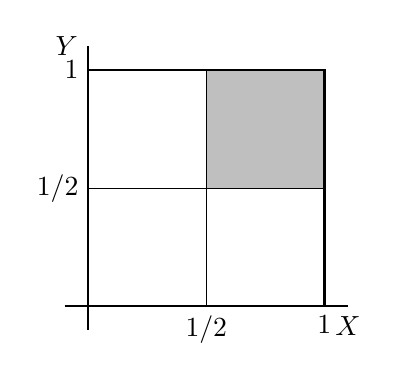
\begin{tikzpicture}[
    scale=3,
    %axis/.style={very thick, ->, >=stealth'},
    important line/.style={thick},
    dashed line/.style={dashed, thin},
    pile/.style={thick, ->, >=stealth', shorten <=2pt, shorten
    >=2pt},
    every node/.style={color=black}
    ]
    % axis
    \draw[thick] (-0.1,0)  -- (1.1,0) node(xline)[below]
        {$X$};
    \draw[thick] (0,-0.1) -- (0,1.1) node(yline)[left] {$Y$};
    % Values
    \draw (0,1) node(xline)[left]{$1$};
    \draw (0,0.5) node(xline)[left]{$1/2$};
    \draw (1,0) node(xline)[below]{$1$};
    \draw (0.5,0) node(xline)[below]{$1/2$};
    % Fill
    \fill[fill=gray!50] (0.5,0.5) -- (0.5,1) -- (1,1) -- (1,0.5) -- cycle;
    % Box
    \draw[important line] (0,0) -- (0,1) -- (1,1) -- (1,0) -- cycle;
    % Lines
    \draw (0.5,0) coordinate (A) -- (0.5,1);
    \draw (0,0.5) coordinate (C) -- (1,0.5);
\end{tikzpicture}  
\end{minipage}%
\begin{minipage}[t]{0.3\textwidth}
    \centering 
    %%%%%%%%%%%%%%%%%%%%%%%%%%%%%%%%%%%%%%% P(Z > 1/4)
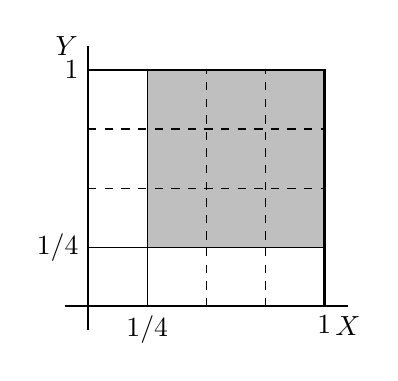
\begin{tikzpicture}[
    scale=3,
    %axis/.style={very thick, ->, >=stealth'},
    important line/.style={thick},
    dashed line/.style={dashed, thin},
    pile/.style={thick, ->, >=stealth', shorten <=2pt, shorten
    >=2pt},
    every node/.style={color=black}
    ]
    % axis
    \draw[thick] (-0.1,0)  -- (1.1,0) node(xline)[below]
        {$X$};
    \draw[thick] (0,-0.1) -- (0,1.1) node(yline)[left] {$Y$};
    % Values
    \draw (0,1) node(xline)[left]{$1$};
    \draw (0,0.25) node(xline)[left]{$1/4$};
    \draw (1,0) node(xline)[below]{$1$};
    \draw (0.25,0) node(xline)[below]{$1/4$};
    % Fill
    \fill[fill=gray!50] (0.25,0.25) -- (0.25,1) -- (1,1) -- (1,0.25) -- cycle;
    % Box
    \draw[important line] (0,0) -- (0,1) -- (1,1) -- (1,0) -- cycle;
    % Lines
    \draw (0.25,0) coordinate (A) -- (0.25,1);
    \draw[style=dashed] (0.5,0) coordinate (A) -- (0.5,1);
    \draw[style=dashed] (0.75,0) coordinate (A) -- (0.75,1);
    \draw (0,0.25) coordinate (C) -- (1,0.25);
    \draw[style=dashed] (0,0.5) coordinate (C) -- (1,0.5);
    \draw[style=dashed] (0,0.75) coordinate (C) -- (1,0.75);
\end{tikzpicture}
\end{minipage}%
\begin{minipage}[t]{0.3\textwidth}
    \centering
    %%%%%%%%%%%%%%%%%%%%%%%%%%%%%%%%%%%%%%% P(Z > 3/4)
    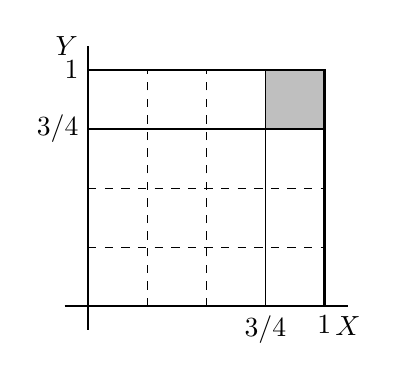
\begin{tikzpicture}[
        scale=3,
        %axis/.style={very thick, ->, >=stealth'},
        important line/.style={thick},
        dashed line/.style={dashed, thin},
        pile/.style={thick, ->, >=stealth', shorten <=2pt, shorten
        >=2pt},
        every node/.style={color=black}
        ]
        % axis
        \draw[thick] (-0.1,0)  -- (1.1,0) node(xline)[below]
            {$X$};
        \draw[thick] (0,-0.1) -- (0,1.1) node(yline)[left] {$Y$};
        % Values
        \draw (0,1) node(xline)[left]{$1$};
        \draw (0,0.75) node(xline)[left]{$3/4$};
        \draw (1,0) node(xline)[below]{$1$};
        \draw (0.75,0) node(xline)[below]{$3/4$};
        % Fill
        \fill[fill=gray!50] (0.75,0.75) -- (0.75,1) -- (1,1) -- (1,0.75) -- cycle;
        % Box
        \draw[important line] (0,0) -- (0,1) -- (1,1) -- (1,0) -- cycle;
        % Lines
        \draw[style=dashed] (0.25,0) coordinate (A) -- (0.25,1);
        \draw[style=dashed] (0.5,0) coordinate (A) -- (0.5,1);
        \draw (0.75,0) coordinate (A) -- (0.75,1);
        \draw[style=dashed] (0,0.25) coordinate (C) -- (1,0.25);
        \draw[style=dashed] (0,0.5) coordinate (C) -- (1,0.5);
        \draw (0,0.75) coordinate (C) -- (1,0.75);
    \end{tikzpicture}
\end{minipage}
\end{figure}
If we simulate lots of $X$ and $Y$ values, we see that about 1/4th of them will have both $X$ and
$Y$ values larger than 1/2, so $\P(Z>1/2) = 1/4$. Similarly, we get $\P(Z>1/4) = 9/16$ and
$\P(Z > 3/4) = 1/16$. Confirming this with a simulation.

\begin{lstlisting}[style=RSyntax]
# 2.7 - Simulating U(0,1)
N = 100000;X = runif(N);Y = runif(N)

Z = pmin(X, Y) # This is: Z = min{X, Y}

# Comparing simualted vs. theoretical results
sum(Z > 0.5)/N
1/4
sum(Z > 0.25)/N
9/16
sum(Z > 0.75)/N
1/16   
\end{lstlisting}
\begin{Verbatim}[fontsize=\small]
> # Comparing simualted vs. theoretical results
> sum(Z > 0.5)/N
[1] 0.24888
> 1/4
[1] 0.25

> sum(Z > 0.25)/N
[1] 0.56156
> 9/16
[1] 0.5625

> sum(Z > 0.75)/N
[1] 0.06205
> 1/16
[1] 0.0625
\end{Verbatim}

\newpage\noindent
By inspecting the images on the previous page, we can determine the 'shape' of the probabilities.
For $Z > 1/4$ we remove the union of $X \leq 1/4$ and $Y\leq 1/4$. We define $A = \{X \leq z\}$ and
$B = \{Y\leq z\}$, and can write the general case as:
\begin{align*}
    \P(Z > z) &=
    1 - \P(\{X \leq z\}\cup \{Y \leq z\}) \\
    &= 1 - \P(A\cup B) \\
    &= 1 - \big[\P(A) + \P(B) - \P(A\cap B)\big] \\
    &= 1 - \big[\P(A) + \P(B) - \P(A)\P(B)\big]
\end{align*}
Where we used Lemma 1.6, and the fact that $X$ and $Y$ are independent. By using the probability
law of complements, we can find the expression for $\P(Z\leq z)$.
$$
\P(Z\leq z) = \P(X\leq z) + \P(Y\leq z) - \P(X\leq z)\P(Y\leq z)
$$
The CDF for a uniform distribution on $U(a,b)$ is:
$$
F(z) = \frac{z-a}{b-a} \imp F_X(z) = F_Y(z) = \frac{z-0}{1-0} = z
$$
Which means:
$$
F_Z(z) = F_X(z) + F_Y(z) - F_X(z)F_Y(z) = 2z - z^2
$$
We can confirm our illustrations and simulated examples again by noting that:
\begin{align*}
    F_Z(1/2) &= \frac{1}{2} + \frac{1}{2} - \left(\frac{1}{2}\cdot\frac{1}{2}\right) = 1 - \frac{1}{4} = \frac{3}{4} \\
    F_Z(1/4) &= \frac{1}{4} + \frac{1}{4} - \left(\frac{1}{4}\cdot\frac{1}{4}\right) = \frac{8}{16} - \frac{1}{16} = \frac{7}{16}\\
    F_Z(3/4) &= \frac{3}{4} + \frac{3}{4} - \left(\frac{3}{4}\cdot\frac{3}{4}\right) = \frac{24}{16} - \frac{9}{16} = \frac{15}{16}
\end{align*}
which gives us the opposite results as expected (since we simulated and illustrated $\P(Z > z)$).
The PDF $f_Z(z)$ is the derivative of $F_Z(z)$.
Including PDF-plot and histogram of the simulated $Z$s.
$$
f_Z(z) = \frac{d}{dz}\Big(F_Z(z)\Big) = 2 - 2z.
$$
%Including a plot of the PDF as well as the histogram of the simulated $Z$ values.
\begin{figure}[H]
    \begin{minipage}{0.5\textwidth}
\begin{tikzpicture}
    \begin{axis}[
        width=0.8\textwidth,
        axis lines = left,
        ymin = -0.002,
        ymax = 2.1,
        xlabel = $z$,
        ylabel = {$f_Z(z)$},
    ]
    %Section 1
    \addplot [
        domain=0:1, 
        samples=10, 
        color=blue,
        style=ultra thick,
    ]
    {2 - 2*x};
    \end{axis}
\end{tikzpicture}
    \end{minipage}
    \begin{minipage}{0.5\textwidth}
        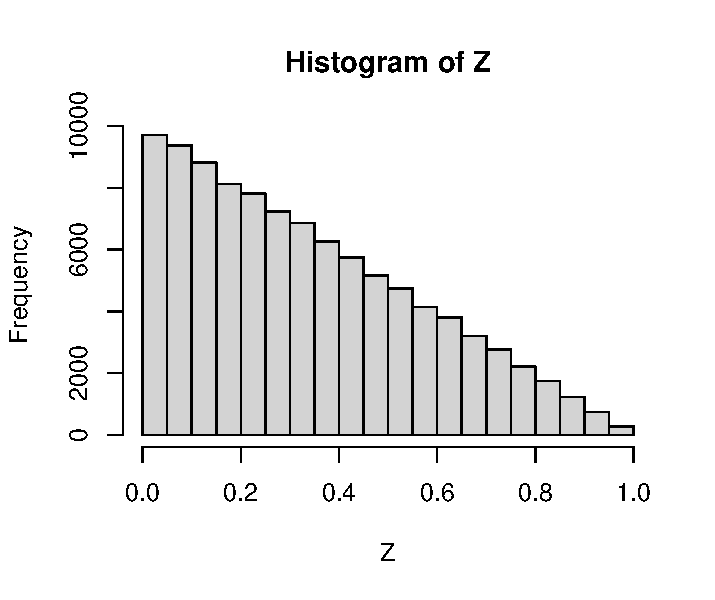
\includegraphics[scale=0.55]{ch2_2.7b.pdf}
    \end{minipage}
\end{figure}

\newpage\noindent
%%%%%%%%%%%%%%%%%%%%%%%%%%%%%%%%%%%%%%%%%%%%%%%%%%%%%%%%%%%%%%%%%%%%%%%%%%%%%%%
\textbf{2.8}\\  % PDF page 45
The RV $X$ has CDF $F$. Finding the CDF of $X^+ = \max\{0, X\}$.

\medskip\noindent
From the definition of CDF:
\begin{align*}
    F_{X^+}(u) &=  \P\big(\max(0, X)\leq u\big)\\
    &= \P\Big(\{\omega\in \Omega \;:\; X(\omega)\leq u\;\text{and}\; u\geq 0\}\Big)
\end{align*}
We must consider two cases. When $u < 0$:
\begin{align*}
    F_{X^+}(u) &= \P\Big(\{\omega\in \Omega \;:\; X(\omega)\leq u\;\text{and}\; u\geq 0\}\Big) \\
    &= \P(\emptyset) \\
    &= 0
\end{align*}
When $u\geq 0$:
\begin{align*}
    F_{X^+}(u) &= \P\Big(\{\omega\in \Omega \;:\; X(\omega)\leq u\;\text{and}\; u\geq 0\}\Big) \\
    &= \P\Big(\{\omega\in \Omega \;:\; X(\omega)\leq u\}\Big)  \\
    &= \P(X\leq u) \\
    &= F_X(u)
\end{align*}
So in summary:
$$
F_{X^+}(u) =
\left\{
    \begin{matrix}
        0 & u<0 \\
        F_X(u) & u\geq0 \\
    \end{matrix}
\right.
$$

% \medskip\noindent
% Illustration of what happens when we go from $X$ to $X^+$ for some continuous
% distribution, such as $X\sim N(0,1)$.
% \begin{figure}[H]
%     \begin{minipage}{0.5\textwidth}
% \begin{tikzpicture}
%     \begin{axis}[
%         width=\textwidth,
%         axis lines = left,
%         ymin = -0.002,
%         ymax = 0.5,
%         xlabel = $x$,
%         ylabel = {$f_X(x)$},
%     ]
%     %Section 1
%     \addplot [
%         domain=-2:2, 
%         samples=50, 
%         color=blue,
%         style=ultra thick,
%     ]
%     {1/(sqrt(2*3.1415))*exp(-0.5*x^2)};
%     \end{axis}
% \end{tikzpicture}
%     \end{minipage}
%     \begin{minipage}{0.5\textwidth}
%         \begin{tikzpicture}
%             \begin{axis}[
%                 width=\textwidth,
%                 axis lines = left,
%                 ymin = -0.002,
%                 ymax = 0.5,
%                 xlabel = $x$,
%                 ylabel = {$f_{X^+}(x)$},
%             ]
%             %Section 1
%             \addplot [
%                 domain=-2:0, 
%                 samples=2, 
%                 color=blue,
%                 style=ultra thick,
%             ]
%             {0};
%             %Section 2
%             \addplot [
%                 domain=0:2, 
%                 samples=50, 
%                 color=blue,
%                 style=ultra thick,
%             ]
%             {1/(sqrt(2*3.1415))*exp(-0.5*x^2)};
%             %Vertical lines
%             \addplot +[mark=none, color=blue] coordinates {(0, -0) (0, 0.4)};
%             \end{axis}
%         \end{tikzpicture}
%     \end{minipage}
% \end{figure}
% We split up the $X$ into negative and positive values, which becomes a disjoint set.
% $$
% \{X\leq x : x\in\R\} = 
% \{X\leq x : x\leq 0\} \cup \{0 < X\leq x : x>0\}
% $$
% Since they are disjoint:
% $$
% \P(X\leq x) = \P(X \leq 0) + \P(0<X\leq x) = F(0) + F(x) - F(0)
% $$
% We can split up the CDF:
% $$
% F(X\leq x) = F(X\leq 0)
% $$
% \medskip\noindent
% One of the defining properties of a PDF is that it must be greater than or equal to 0.
% Since the CDF if the integral of the PDF, it will always be greater than or equal to 0
% as well.
%%%% No, wait - this is incorrect. We could have e.g. U(-1, 1) or N(0, 1) in which case many
%%%% X will be negative. So the PDF is never negative, that is true, but that says
%%%% nothing about the X.

\bigskip\noindent
%%%%%%%%%%%%%%%%%%%%%%%%%%%%%%%%%%%%%%%%%%%%%%%%%%%%%%%%%%%%%%%%%%%%%%%%%%%%%%%
\textbf{2.9}\\  % PDF page 45
We have $X\sim \text{Exp}(\beta)$. The PDF is given by:
$$
f(x) = \frac{1}{\beta}e^{-x/\beta},\quad x > 0
$$
Finding the CDF by integrating the PDF.
\begin{align*}
    F(y) &= \int_{-\infty}^y f(x)dx \\
    &= \frac{1}{\beta}\int_0^y e^{-x/\beta}dx\\
    &= \frac{1}{\beta}\big[-\beta e^{-x/\beta}\big]_0^y\\
    &= \big[-e^{-x/\beta}\big]_0^y \\
    &= 1 - e^{-y/\beta}
\end{align*}
To find the inverse $F^{-1}(q)$ we set $q = F(y)$ and solve for $y$.
$$
q = 1 - e^{-y/\beta}
\imp
y = -\beta\log(1 - q)
\imp
F^{-1}(q) = -\beta\log(1 - q)
$$

\bigskip\noindent
%%%%%%%%%%%%%%%%%%%%%%%%%%%%%%%%%%%%%%%%%%%%%%%%%%%%%%%%%%%%%%%%%%%%%%%%%%%%%%%
\textbf{2.10}\\  % PDF page 45
If $X$ and $Y$ are independent, then $g(X)$ and $h(Y)$ are independent for some functions
$g$ and $h$.

\medskip\noindent
\textsc{Proof}.
Let $X$ and $Y$ be some arbitrary random variables, and let $x$ and $y$ be
values in the range of $g$ and $h$ such that $g(X) = x$ and $h(Y) = y$. Then:
\begin{align*}
    \P(g(X) = x, h(Y) = y) &=
    \P(X = g^{-1}(x), Y = h^{-1}(y)) \\
\shortintertext{By independence of $X$ and $Y$.}
&= \P(X = g^{-1}(x))\P(Y = h^{-1}(y)) \\
&= \P(g(X) = x)\P(h(Y) = y) 
\end{align*}
which shows that $g$ and $h$ satisfies the condition for independence.\qed
% When $X$ and $Y$ are independent, we want to show that the following is true:
% $$
% \P(g(X)\cap h(Y)) = \P(g(X))\P(h(Y))
% $$

\bigskip\noindent
%%%%%%%%%%%%%%%%%%%%%%%%%%%%%%%%%%%%%%%%%%%%%%%%%%%%%%%%%%%%%%%%%%%%%%%%%%%%%%%
\textbf{2.11}\\  % PDF page 45
Tossing a coin which has probability $p$ of getting H. We let $X$ denote the
number of heads and $Y$ the number of tails.

\medskip\noindent(a) Showing that $X$ and $Y$ are dependent. First it will be helpful
to consider a simplified case where we have $N=1$ and $N=2$ coin tosses, and assuming $p=1/2$.
\begin{figure}[H]
    \begin{minipage}{0.5\textwidth}
        $N = 1$ Tosses \\
        $$
            \begin{tabular}{c|c|c|c}
                & $Y=0$ & $Y=1$ & \\
                \hline
                $X=0$ & 0 & $1/2$ & $1/2$ \\
                \hline
                $X=1$ & $1/2$ & 0 & $1/2$ \\
                \hline
                & $1/2$ & $1/2$ & 1
            \end{tabular}
        $$
        \rule{0pt}{5pt}
    \end{minipage}
    \begin{minipage}{0.5\textwidth}
        $N = 2$ Tosses \\
        $$
            \begin{tabular}{c|c|c|c|c}
                & $Y=0$ & $Y=1$ & $Y=2$ & \\
                \hline
                $X=0$ & 0 & 0 & 1/4 & $1/4$ \\
                \hline
                $X=1$ & 0 & 1/2 & 0 & $1/2$ \\
                \hline
                $X=2$ & $1/4$ & 0 & 0 & $1/4$ \\
                \hline
                & $1/4$ & $1/2$ & $1/4$ & 1
            \end{tabular}
        $$
    \end{minipage}
\end{figure}
In the case of $N=2$, we see that $f(0, 2) = 1/4$ while $f_X(0)f_Y(2) = 1/16$. This will be the
inspiration for how we show it in the general case with $N$ tosses and probability $p$ of heads.

\medskip\noindent
We only need to show one specific case where $\P(X=x, Y=y) \not= \P(X=x)\P(Y=y)$ to show that these
values are dependent. The total number of tosses will be $N = X + Y$ and we compare the cases where
we get $N$ heads. In that case, using the Multinomial distribution:
$$
\P(X=N, Y=0) = {N\choose N,0} =p^N(1-p)^0 = p^N,
$$
but with the two Binomial distributions:
$$
\P(X=N)\P(Y=0) = {N\choose N}p^N(1-p)^0\times {N\choose 0}p^0(1-p)^N = p^N(1-p)^N.
$$
These are not equal, showing that $X$ and $Y$ are dependent variables.


\newpage\noindent
%%%%%%%%%%%%%%%%%%%%%%%%%%%%%%%%%%%%%%%%%%%%%%%%%%%%%%%%%%%%%%%%%%%%%%%%%%%%%%%
(b) Now we have $N\sim\text{Poisson}(\lambda)$, where $N = X + Y$ for $X$ heads
and $Y$ tails. Show that these values are now independent.

\medskip\noindent\emph{Current solution, but not sure it's correct...}\\
Assuming $X=x$ and $Y=y$. Then:
\begin{align*}
    \P(X=x\cap Y=y) &= \P(X=x\cap Y=y\cap N = x+y) \\
    &= \P(X=x\cap Y=y \mid N = x+y)\cdot\P(N = x+y) \\
    &= {x+y\choose x}p^x(1-p)^y\cdot e^{-\lambda}\frac{\lambda^{x+y}}{(x+y)!} \\
    &= \frac{\cancel{(x+y)!}}{x!y!}p^x(1-p)^y\cdot e^{-\lambda}\frac{\lambda^x\lambda^y}{\cancel{(x+y)!}} \\
    &= e^{-\lambda}\frac{p^x\lambda^x}{x!}\cdot\frac{(1-p)^y\lambda^y}{y!} \\
    &= e^{-\lambda p}\frac{p^x\lambda^x}{x!}\cdot e^{-\lambda(1-p)}\frac{(1-p)^y\lambda^y}{y!} \\
    &= \P(X=x | \lambda p)\cdot\P(Y=y|\lambda(1-p)) \\
    &= \P(X=x)\P(Y=y)
\end{align*}
Which shows we have independence. We used:
$$
e^{-\lambda} = e^{-\lambda(p - p + 1)} = e^{-\lambda p + \lambda p - \lambda}
= e^{-\lambda p}e^{\lambda p - \lambda} = e^{-\lambda p}e^{-\lambda(1-p)}.
$$
Also, we made the assumption that $\P(X=x\cap Y=y \mid N = x+y)$ is Binomial. But I think this is
only true when we can assume that $X$ and $Y$ are independent... which is what we are trying to show.
Will review this later... hopefully!

\bigskip\noindent
%%%%%%%%%%%%%%%%%%%%%%%%%%%%%%%%%%%%%%%%%%%%%%%%%%%%%%%%%%%%%%%%%%%%%%%%%%%%%%%
\textbf{2.12} \textsc{Theorem} 2.33\\  % PDF page 45
Suppose that the range of $X$ and $Y$ is a (possibly infinite)
rectangle. If $f(x, y) = g(x)h(y)$ for some functions $g$ and $h$ (not necessarily
probability density functions) then $X$ and $Y$ are independent.

\medskip\noindent\textsc{Proof}. From the joint PDF, we can find the marginal distributions:
$$
f_X(x) = \int f(x, y) dy, \quad
f_Y(y) = \int f(x, y) dx
$$
By applying these integrals to both sides of the equality:
$$
\int f(x, y) dy = g(x)\int h(y) dy \imp f_X(x) = g(x)
$$
$$
\int f(x, y) dx = h(y)\int g(x) dx \imp f_Y(y) = h(y)
$$
We get $g(x)$ and $h(y)$ since they are equal to $f(x,y)$ over the entire 'rectangle' and must therefore
integrate to 1. This leaves us with: $f(x, y) = g(x)h(y) = f_X(x)f_Y(y)$, and by the results in exercise 2.5,
this means that $X$ and $Y$ are independent. \qed

\newpage\noindent
%%%%%%%%%%%%%%%%%%%%%%%%%%%%%%%%%%%%%%%%%%%%%%%%%%%%%%%%%%%%%%%%%%%%%%%%%%%%%%%
\textbf{2.13}\\  % PDF page 45
(a) Finding the PDF of $Y = e^X$ when $X\sim N(0,1)$.
\begin{align*}
    F_Y(y) &= \P(Y\leq y) = \P(e^X \leq y) \\
    &= \P(X\leq \log(y)) = F_X(\log(y))
\end{align*}
We simply get the standard normal distribution back, but we input the logarithm of $y$.
This means we get the PDF:
$$
f_Y(y) = f_X(\log(y)) = \frac{1}{\sqrt{2\pi}}\exp\left(-\frac{1}{2}\big(\log(y)\big)^2\right)
$$
Plotting the function:
\begin{figure}[H]
\begin{minipage}{0.5\textwidth}
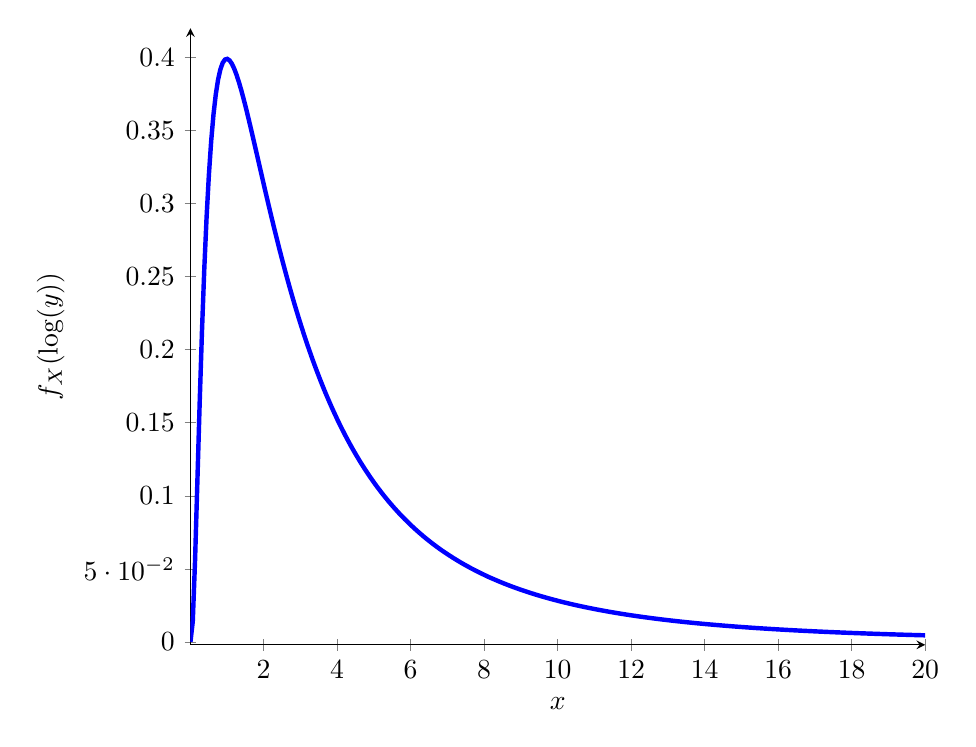
\begin{tikzpicture}
    \begin{axis}[
        width=0.9\textwidth,
        axis lines = left,
        ymin = -0.002,
        ymax = 0.42,
        xlabel = $x$,
        ylabel = {$f_X(\log(y))$},
    ]
    %Section 1
    \addplot [
        domain=-5:20, 
        %domain=-1:5, 
        samples=400, 
        color=blue,
        style=ultra thick,
    ]
    {(1/(sqrt(2*pi)))*exp(-0.5*ln(x)*ln(x))};
    \end{axis}
\end{tikzpicture}
\end{minipage}
\begin{minipage}{0.5\textwidth}
\end{minipage}
\end{figure}
(b) Plotting histogram of simulated results. Comparable to the plot above.
\begin{figure}[H]
    \begin{minipage}{0.5\textwidth}
        \begin{center}
            \begin{figure}[H]
            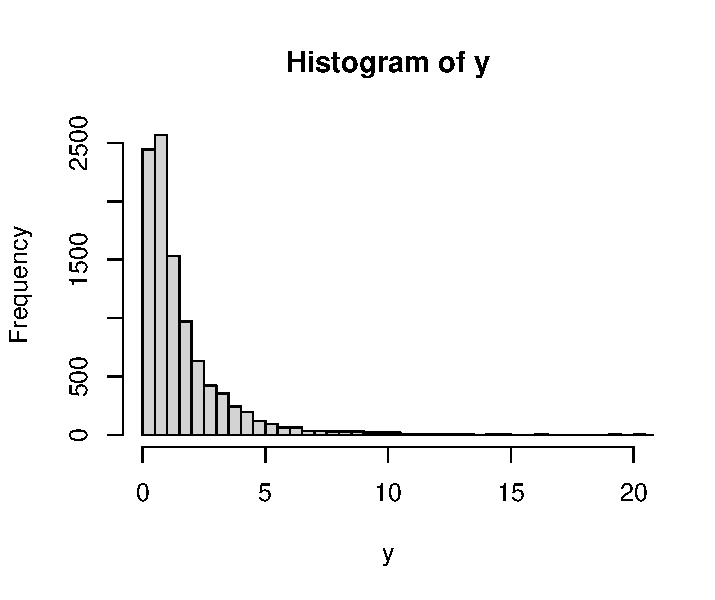
\includegraphics[scale=0.65]{ch2_2.13b.pdf}
            \end{figure}
        \end{center}
    \end{minipage}
    \begin{minipage}{0.5\textwidth}
    \begin{lstlisting}[style=RSyntax]
x = rnorm(10000)
y = exp(x)
hist(y, breaks = 100, xlim = c(0, 20))
pdf("~/AllStatistics/files/ch2_2.13b.pdf",
     width = 4.7747, height = 4)
hist(y, breaks = 100, xlim = c(0, 20))
dev.off()
    \end{lstlisting}
    \rule{0pt}{55pt}
\end{minipage}
\end{figure}






\begin{comment}

\bigskip\noindent
%%%%%%%%%%%%%%%%%%%%%%%%%%%%%%%%%%%%%%%%%%%%%%%%%%%%%%%%%%%%%%%%%%%%%%%%%%%%%%%
\textbf{2.X}\\  % PDF page 45


\begin{align*}
    A &= B
\end{align*}


\begin{equation*}
    A = B
    \tag*{\qed}
\end{equation*}


%%% Tikz Image - side by side
\begin{figure}
    \begin{minipage}[0.5\textwidth]
\begin{tikzpicture}
    \begin{axis}[
        width=\textwidth,
        axis lines = left,
        ymin = -0.002,
        ymax = 2.1,
        xlabel = $z$,
        ylabel = {$f_Z(z)$},
    ]
    %Section 1
    \addplot [
        domain=0:1, 
        samples=10, 
        color=blue,
        style=ultra thick,
    ]
    {2 - 2*x};
    \end{axis}
\end{tikzpicture}
    \end{minipage}
    \begin{minipage}[0.5\textwidth]
\begin{tikzpicture}
    \begin{axis}[
        width=\textwidth,
        axis lines = left,
        ymin = -0.002,
        ymax = 2.1,
        xlabel = $z$,
        ylabel = {$f_Z(z)$},
    ]
    %Section 1
    \addplot [
        domain=0:1, 
        samples=10, 
        color=blue,
        style=ultra thick,
    ]
    {2 - 2*x};
    \end{axis}
\end{tikzpicture}
    \end{minipage}
\end{figure}


\begin{lstlisting}[style=RSyntax, title=R]
# Code
\end{lstlisting}

\begin{verbatim}
# Output
\end{verbatim}


\end{comment}